\documentclass{beamer}

\usepackage[utf8]{inputenc}
\usepackage{default}
\usepackage{graphicx}
\usepackage{verbatim}
\usepackage{tikz}
\usepackage{color}
\usepackage{chemfig}
\usetheme{Szeged}
\usecolortheme{seahorse}

\useinnertheme{rounded}
\title{\textbf{HUFFMAN CODING}}

\subtitle{A Greedy Approach}
\author{Badhan Das\\
	Zarin Tasnim Promi}
\institute{Bangladesh University of Engineering and Technology}
\titlegraphic{
\includegraphics[width=1.5cm]{BuetLogo.png}}

\begin{document}
\begin{frame}
\titlepage
\end{frame}

\begin{frame}
\frametitle{\textbf{Traditional Encoding}}
\begin{itemize}
 \item Characters are typically encoded by their ASCII codes with 8 bits per character.  
 \item As example the word 'ABC' takes 24 bits to encode,
\end{itemize}

\end{frame}




\begin{frame}
\frametitle{\textbf{A Common Scenerio}}
\begin{itemize}
 \item Memory Restrictions
 \item Multiple file sending Restrictions
\end{itemize}
\begin{figure}
  
\includegraphics[width=3cm]{Z.png}
  %\caption{Text Compression}
  %\label{fig:Text Compression}
\end{figure}
\end{frame}

\begin{frame}
\frametitle{\textbf{Solution}}
\begin{itemize}
 \item Text Compression by Implementing Huffman Coding
\end{itemize}
\begin{figure}
  
\includegraphics[width=3cm]{zip2.png}
  \caption{Text Compression}
  \label{fig:Text Compression}
\end{figure}
\end{frame}

\begin{frame}
\frametitle{\textbf{Huffman Coding}}
\begin{itemize}
\item Variable length representation based on symbol frequency
 \pause\item Efficient when symbol probabilities vary widely
 \pause\item Capable of saving 20\% to 90\% space
 \pause\item Uses an optimal encoding tree to determine the code words and vice-versa
\end{itemize}
\end{frame}

\begin{frame}
\frametitle{\textbf{Main Idea}}
 \begin{itemize}
  \item Use fewer bits to represent frequent symbols 
  \item Use more bits to represent infrequent symbols 
 \end{itemize}
 \begin{center}
\begin{tabular}{|   p{2cm}  |  p{2cm}  |  p{2cm}  |  p{2cm}  |}
 \hline
  A  & A & B & A\\
 \hline
\end{tabular} 
\end{center} 
\begin{center}
$ \Downarrow$
\end{center}
\begin{center}
\begin{tabular}{| p{1cm} | p{1cm} | p{2cm} | p{1cm} |}
 \hline
  A & A & B & A\\
 \hline
\end{tabular} 
\end{center} 
\end{frame}

\begin{frame}
  \frametitle{\textbf{Huffman Binary tree Construction}}
   \textcolor{blue}{Steps:}
  \begin{itemize}
   \item Frequency table construction
\item Sorting the table
\item Adding the lowest two frequency 
\item Denoting a new symbol and updating the table
\item Have to repeat the last 3 process until there is one node
\item Performing  a traversal of the tree to obtain new code words
\item Going left is a 0 going right is a 1
\end{itemize}

\end{frame}

\begin{frame}
 \frametitle{\textbf{Huffman Encoding}}
 \begin{itemize}
  \item Encodes high-frequency characters with short code words
  \item Uses an optimal frequency tree to determine the code words
 \end{itemize}
\end{frame}

\begin{frame}
 \frametitle{\textbf{Huffman Encoding Simulation}}
 \textcolor{blue}{EXAMPLE : } \textbf{TELL THE TRUTH}
 \\
 \textcolor{blue}{Frequency Table : }
 \begin{center}
\begin{tabular}{| c | c |}
 \hline
  \textcolor{blue}{Symbol} & \textcolor{blue}{Frequency} \\ \hline  
  T & 4 \\ \hline
 E & 2 \\ \hline  
 H & 2 \\ \hline  
  L & 2 \\ \hline 
   R & 1 \\ \hline  
    U & 1 \\ \hline  
\end{tabular} 
\end{center} 
\end{frame}


\begin{frame}
\frametitle{\textbf{Huffman Encoding Simulation}}

 
\begin{tabular}{| p{0.25cm} | p{0.25cm} | p{0.25cm} | p{0.25cm} | p{0.25cm} | p{0.25cm} | p{0.25cm} | p{0.25cm} | p{0.25cm} | p{0.25cm} | p{0.25cm} |}

\cline{1-1} \cline{3-3} \cline{5-5} \cline{7-7} \cline{9-9} \cline{11-11}

 T && E & & L & & H & & R & & U \\

\cline{1-1} \cline{3-3} \cline{5-5} \cline{7-7} \cline{9-9} \cline{11-11}

\end{tabular} 

\begin{tabular}{p{0.25cm} p{0.25cm} p{0.25cm} p{0.25cm} p{0.25cm} p{0.25cm} p{0.25cm} p{0.25cm} p{0.25cm} p{0.25cm} p{0.25cm}}

4 & & 2 & & 2 & & 2 & & 1 & & 1\\
 
\end{tabular} 
\end{frame}


\begin{frame}

\frametitle{\textbf{Huffman Encoding Simulation}}


 \begin{tabular}{| p{0.25cm} | p{0.25cm} | p{0.25cm} | p{0.25cm} | p{0.25cm} | p{0.25cm} | p{0.25cm} | p{0.25cm} | p{0.25cm} | p{0.25cm} |}

\cline{1-1} \cline{3-3} \cline{5-5} \cline{7-7} \cline{9-9} \cline{11-11}

 T && E & & L & & H & & N1\\

\cline{1-1} \cline{3-3} \cline{5-5} \cline{7-7} \cline{9-9} \cline{11-11}
\end{tabular} 


\begin{tabular}{ p{0.25cm} p{0.25cm} p{0.25cm} p{0.25cm} p{0.25cm} p{0.25cm} p{0.25cm} p{0.25cm} p{0.25cm}}
4 & & 2 & & 2 & & 2 & & 2
 \end{tabular}  


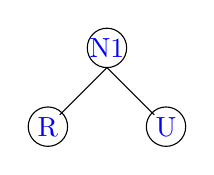
\begin{tikzpicture}
%\draw[red, dashed, very thick, rotate=-135]   (1,7) -- (0,7) -- (0,8);
%\draw (0,-0.5) -- (0,0) -- (0.5,0) -- (0.5,-0.5)-- cycle node{U} ;
\draw  (-0.6,-.85) -- (0,-0.25) -- (0.6,-.85) (0,0) circle[radius=0.25] node{\textcolor{blue}{N1}} (0.75,-1)circle[radius=0.25] node{\textcolor{blue}{U}} (-0.75,-1)circle[radius=0.25] node{\textcolor{blue}{R}};
\end{tikzpicture}

  \end{frame}



\begin{frame}
\frametitle{\textbf{Huffman Encoding Simulation}}


\begin{tabular}{| p{0.25cm} | p{0.25cm} | p{0.25cm} | p{0.25cm} | p{0.25cm} | p{0.25cm} | p{0.25cm} | }

\cline{1-1} \cline{3-3} \cline{5-5} \cline{7-7}

 T & & N2 & & L & & E  \\

\cline{1-1} \cline{3-3} \cline{5-5} \cline{7-7}
\end{tabular}

\begin{tabular}{ p{0.25cm} p{0.25cm} p{0.25cm} p{0.25cm} p{0.25cm} p{0.25cm} p{0.25cm} p{0.25cm} p{0.25cm}}
4 & & 4 & & 2 & & 2 \\
 \end{tabular}  
\\
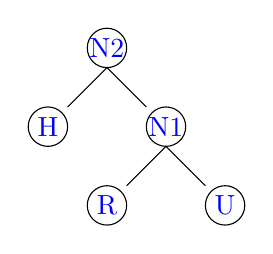
\begin{tikzpicture}
\draw  (-0.5,-.75) -- (0,-0.25) -- (0.5,-.75) (0,0) circle[radius=0.25] node{\textcolor{blue}{N2}} 
(0.75,-1)circle[radius=0.25] node{\textcolor{blue}{N1}} (-0.75,-1)circle[radius=0.25] node{\textcolor{blue}{H}} (0.25,-1.75) -- (0.75,-1.25) -- (1.25,-1.75)
(0,-2) circle[radius=0.25] node{\textcolor{blue}{R}}  (1.5,-2) circle[radius=0.25] node{\textcolor{blue}{U}};
\end{tikzpicture}
\end{frame}


\begin{frame}
\frametitle{\textbf{Huffman Encoding Simulation}}


\begin{tabular}{| p{0.25cm} | p{0.25cm} | p{0.25cm} | p{0.25cm} | p{0.25cm} | }

\cline{1-1} \cline{3-3} \cline{5-5} 

 T & & N2 & & N3   \\

\cline{1-1} \cline{3-3} \cline{5-5}
\end{tabular}

\begin{tabular}{ p{0.25cm} p{0.25cm} p{0.25cm} p{0.25cm} p{0.25cm} p{0.25cm} p{0.25cm}}
4 & & 4 & & 4  \\
 \end{tabular}  
\\

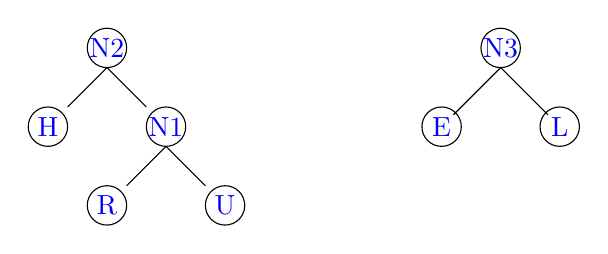
\begin{tikzpicture}
\draw  (-0.5,-.75) -- (0,-0.25) -- (0.5,-.75) (0,0) circle[radius=0.25] node{\textcolor{blue}{N2}} 
(0.75,-1)circle[radius=0.25] node{\textcolor{blue}{N1}} (-0.75,-1)circle[radius=0.25] node{\textcolor{blue}{H}} (0.25,-1.75) -- (0.75,-1.25) -- (1.25,-1.75)
(0,-2) circle[radius=0.25] node{\textcolor{blue}{R}}  (1.5,-2) circle[radius=0.25] node{\textcolor{blue}{U}};
 \draw  (4.4,-.85) -- (5,-0.25) -- (5.6,-.85) (5,0) circle[radius=0.25] node{\textcolor{blue}{N3}} (5.75,-1)circle[radius=0.25] node{\textcolor{blue}{L}} (4.25,-1)circle[radius=0.25] node{\textcolor{blue}{E}};
\end{tikzpicture}


\end{frame}

\begin{frame}
\frametitle{\textbf{Huffman Encoding Simulation}}


\begin{tabular}{| p{0.25cm} | p{0.25cm} | p{0.25cm} |}
\cline{1-1} \cline{3-3} 
N4 & & T  \\
\cline{1-1} \cline{3-3}
\end{tabular}

\begin{tabular}{ p{0.25cm} p{0.25cm} p{0.25cm}}
8 & & 4   \\
\end{tabular}

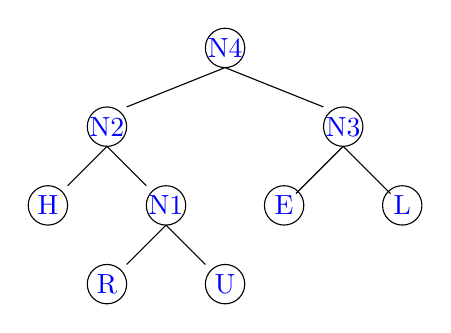
\begin{tikzpicture}
\draw  (-0.5,-.75) -- (0,-0.25) -- (0.5,-.75) (0,0) circle[radius=0.25] node{\textcolor{blue}{N2}} 
(0.75,-1)circle[radius=0.25] node{\textcolor{blue}{N1}} (-0.75,-1)circle[radius=0.25] node{\textcolor{blue}{H}} (0.25,-1.75) -- (0.75,-1.25) -- (1.25,-1.75)
(0,-2) circle[radius=0.25] node{\textcolor{blue}{R}}  (1.5,-2) circle[radius=0.25] node{\textcolor{blue}{U}};
\draw  (2.4,-.85) -- (3,-0.25) -- (3.6,-.85) (3,0) circle[radius=0.25] node{\textcolor{blue}{N3}} (3.75,-1)circle[radius=0.25] node{\textcolor{blue}{L}} (2.25,-1)circle[radius=0.25] node{\textcolor{blue}{E}};
\draw  (0.25,0.25) -- (1.5,0.75) -- (2.75,0.25) (1.5,1) circle[radius=0.25] node{\textcolor{blue}{N4}} ;
\end{tikzpicture}
\end{frame}

\begin{frame}
\frametitle{\textbf{Huffman Encoding Simulation}}
\textcolor{blue}{Step:} Add the last two frequency from the table and denote e new symbol.\\ 

\begin{tabular}{| p{0.25cm} | }
\cline{1-1} 
N5 \\
\cline{1-1}
\end{tabular}

\begin{tabular}{ p{0.25cm} }
12  \\
\end{tabular}

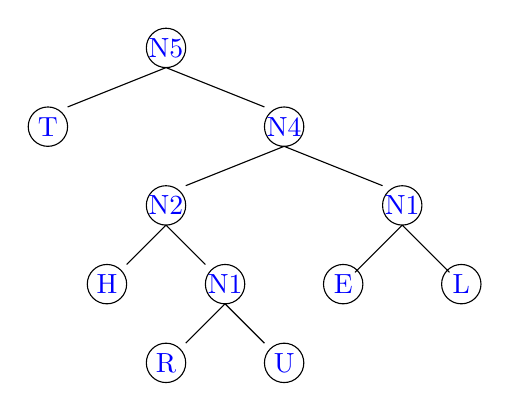
\begin{tikzpicture}
\draw  (-0.5,-.75) -- (0,-0.25) -- (0.5,-.75) (0,0) circle[radius=0.25] node{\textcolor{blue}{N2}} 
(0.75,-1)circle[radius=0.25] node{\textcolor{blue}{N1}} (-0.75,-1)circle[radius=0.25] node{\textcolor{blue}{H}} (0.25,-1.75) -- (0.75,-1.25) -- (1.25,-1.75)
(0,-2) circle[radius=0.25] node{\textcolor{blue}{R}}  (1.5,-2) circle[radius=0.25] node{\textcolor{blue}{U}};
\draw  (2.4,-.85) -- (3,-0.25) -- (3.6,-.85) (3,0) circle[radius=0.25] node{\textcolor{blue}{N1}} (3.75,-1)circle[radius=0.25] node{\textcolor{blue}{L}} (2.25,-1)circle[radius=0.25] node{\textcolor{blue}{E}};
\draw  (0.25,0.25) -- (1.5,0.75) -- (2.75,0.25) (1.5,1) circle[radius=0.25] node{\textcolor{blue}{N4}} ;
\draw  (-1.25,1.25) -- (0,1.75) -- (1.25,1.25) (-1.5,1) circle[radius=0.25] node{\textcolor{blue}{T}} (1.25,1.25) (0,2) circle[radius=0.25] node{\textcolor{blue}{N5}};
\end{tikzpicture}
\end{frame}

\begin{frame}
\frametitle{\textbf{Huffman Encoding Simulation}}
 \begin{figure}
  \includegraphics[width=\linewidth]{pro.png}
  %\caption{Text Compression}
  %\label{fig:Text Compression}
\end{figure}
 
 
\end{frame}


\begin{frame}
\frametitle{\textbf{Decoding Simulation}}
 \begin{figure}
  \includegraphics[width=\linewidth]{decode.png}
  %\caption{Text Compression}
  %\label{fig:Text Compression}
\end{figure}
 
 \end{frame}

\begin{frame}
 \begin{figure}
% ANY QUESTIONS ?
  
\includegraphics[width=5cm]{question.jpg}
  %\caption{Text Compression}
  %\label{fig:Text Compression}
\end{figure}
 
\end{frame}
\begin{frame}
\begin{center}
 
 \textbf{THANK YOU ALL}
 \end{center}
\end{frame}


\end{document}
